\documentclass[aspectratio=169]{beamer}
\usetheme{metropolis}
\usepackage[utf8]{inputenc}
\usepackage[T1]{fontenc}
\usepackage{appendixnumberbeamer}
\usepackage{booktabs}
\usepackage[scale=2]{ccicons}
\usepackage{pgfplots}
\pgfplotsset{compat=1.18}
\usepackage{xspace}

% ── Colours ───────────────────────────────────────────────────────────────────
\definecolor{mLightBrown}{HTML}{EB811B}
\definecolor{mLightGreen}{HTML}{14B03D}
\setbeamercolor{progress bar}{fg=mLightBrown}
\setbeamercolor{alerted text}{fg=mLightBrown}

% ── Metadata ──────────────────────────────────────────────────────────────────
\title{Minimal Beamer Presentation}
\subtitle{Metropolis Theme}
\date{\today}
\author{Alex Johnson}
\institute{Center for Modern Research}
\titlegraphic{\hfill\includegraphics[height=1.5cm]{logo}}

\begin{document}

\maketitle

\begin{frame}{Table of contents}
  \setbeamertemplate{section in toc}[sections numbered]
  \tableofcontents[hideallsubsections]
\end{frame}

\section{Introduction}

\begin{frame}[fragile]{Metropolis}
  The \themename theme is a Beamer theme with minimal visual noise.
  Enable it by loading:
  \begin{verbatim}
  \usetheme{metropolis}
  \end{verbatim}

  Note, that you have to have Mozilla's \emph{Fira Sans} font and XeTeX
  installed to enjoy this theme. If you just want to use it without
  XeTeX, you will need to include the \texttt{[nofont]} option.
\end{frame}

\begin{frame}{Features}
  \begin{columns}[T, onlytextwidth]
    \column{0.5\textwidth}
      \textbf{Design}
      \begin{itemize}
        \item Clean, minimal aesthetic
        \item Focus on content
        \item Modern sans-serif fonts
      \end{itemize}

    \column{0.5\textwidth}
      \textbf{Functionality}
      \begin{itemize}
        \item Progress bar
        \item Section slides
        \item Standout frames
      \end{itemize}
  \end{columns}
\end{frame}

\section{Elements}

\begin{frame}{Typography}
  \begin{itemize}
    \item Regular text looks clean and readable.
    \item \textit{Italic text} for emphasis.
    \item \textbf{Bold text} for key terms.
    \item \texttt{Monospace} for code snippets.
  \end{itemize}

  \vspace{1em}
  \begin{alertblock}{Important Notice}
    Use alert blocks to highlight critical information.
  \end{alertblock}
\end{frame}

\begin{frame}{Figures}
  \begin{figure}
    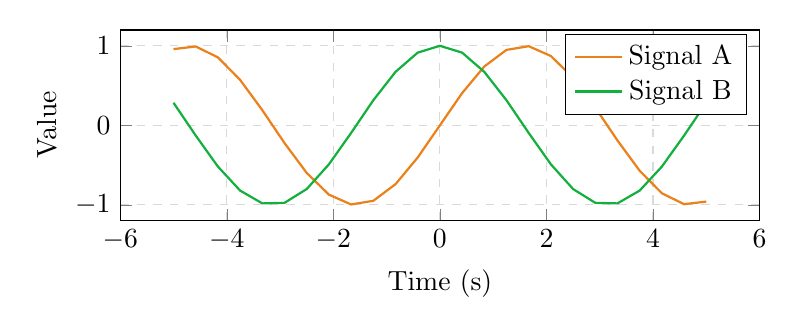
\begin{tikzpicture}
      \begin{axis}[
        width=0.8\textwidth, height=4cm,
        xlabel={Time (s)}, ylabel={Value},
        grid=major, grid style={dashed, gray!30},
      ]
        \addplot[color=mLightBrown, thick] {sin(deg(x))};
        \addplot[color=mLightGreen, thick] {cos(deg(x))};
        \legend{Signal A, Signal B}
      \end{axis}
    \end{tikzpicture}
  \end{figure}
\end{frame}

\section{Conclusion}

\begin{frame}{Summary}
  \begin{itemize}
    \item Metropolis provides a clean, professional look.
    \item Ideal for technical and academic presentations.
    \item Easy to customise with standard Beamer commands.
  \end{itemize}
\end{frame}

\begin{frame}[standout]
  Questions?
\end{frame}

\appendix

\begin{frame}{Backup: Additional Data}
  This frame is in the appendix — page numbers reset here.
\end{frame}

\end{document}
